%&pdflatex

\documentclass[12pt, twoside]{article}

\usepackage{algorithm}
\usepackage{algpseudocode}
\usepackage{amsmath} % for implementation of the matrix environment
\usepackage{blindtext}
\usepackage{caption}
\usepackage{color}
\usepackage[pdftex]{graphicx} \graphicspath{{./figures/}}
\usepackage{epstopdf} \epstopdfsetup{update} % only regenerate pdf files when eps file is newer
\usepackage{float} % figure groups aka floats
\usepackage{forest} % for MFS elimination tree diagram
\usepackage[shellescape,latex]{gmp} % metapost for UMLs
\usepackage[hidelinks]{hyperref} % ToC/LoA/LoF/LoT entries are links

% Figure X instead of X.
% \makeatletter
% \renewcommand{\p@figure}{\figurename\ }
% \makeatother
%

% fig. X instead of X when using \cref
\usepackage[nameinlink]{cleveref}
%

\usepackage{mathptmx} % Times New Roman like font
\usepackage{pdfpages} % for inserting pdf as the initial pages
\usepackage{setspace} \onehalfspacing % 1.5 line spacing
\usepackage{subcaption}
\usepackage{xfrac} % nice slanted fractions
\usepackage{fancyhdr}
\usepackage{titlesec}

% dot after section number in ToC
\makeatletter
\renewcommand\numberline[1]{\hb@xt@\@tempdima{#1.\hfil}}
\makeatother
%

\titlelabel{\thetitle.\quad}
\usepackage[a4paper, width=150mm, top=30mm, bottom=30mm]{geometry}

% Styles for captions
\captionsetup[figure]{labelfont={bf}, textfont={small}}
\captionsetup[subfigure]{labelfont={bf}, textfont={small}}
%

% Custom commands
\newcommand{\mycfoot}{\cfoot{\thepage}}
\newcommand{\todo}[1]{\textcolor{teal}{\textbf{@TODO: }#1}}
\newcommand{\bt}{\blindtext}
\newcommand{\eps}{\varepsilon}
\newcommand{\rev}[1]{\textcolor{red}{\textbf{@REV: }#1}}
% \newcommand{\rev}[1]{#1}
\newcommand{\T}[1]{\texttt{#1}}
%

\algnewcommand\And{\,\textbf{and}\,}
\algnewcommand\Or{\,\textbf{or}\,}
\algnewcommand{\LineComment}[1]{\State \(\triangleright\) #1}

% \include{0-lang-defs}

\renewcommand{\headrulewidth}{0.5pt}
\renewcommand{\footrulewidth}{0.5pt}% default is 0pt



% Styl z samym numerem strony wycentrowanym w stópce

\fancypagestyle{only-cfoot}{
\renewcommand{\headrulewidth}{0pt}
\renewcommand{\footrulewidth}{0pt}
\fancyhead{}
\fancyfoot{
\centering
\thepage
}
% \cfoot{\thepage}
}



% Styl aplikowany jako domyślny
 
\pagestyle{fancy}
\fancyhf{}


% Wydłuża linie w nagłówku i sópce po bokach

% \fancyhfoffset[L]{1cm} % left extra length
% \fancyhfoffset[R]{1cm} % right extra length



% Header

% \lhead{\nouppercase{\leftmark}}
\lhead{\nouppercase{\rightmark}}
% \rhead{\nouppercase{\rightmark}}
\rhead{\textbf{\thepage}}



%Footer

\lfoot{K. Kmiecik \emph{Leveraging container management for scientific computing}}

%%%%%%%% DOCUMENT

\begin{document}


% INITIAL PAGES

\includepdf[pages={-, {}}]{initial-pages-v4.pdf} % `-' for all pages, `{}' for an empty page
% 
\includepdf[pages={-, {}}]{initial-pages-v2.pdf}


%%% KEYWORDS
% DAG scheduling, container, Kubernetes, cloud computing, scientific computing, performance


\cleardoublepage
\thispagestyle{empty}


%%% ACKNOWLEDGMENTS
% \vspace*{\fill}
\begin{center}
\textbf{Acknowledgments}
\end{center}
\begin{center}
\begin{minipage}{0.62\textwidth}
I would like to express my gratitude to my supervisor, dr hab. inż. Bartosz Baliś, prof. AGH, for his guidance, knowledge sharing, and invaluable help with the implementation of a solution used in the experimental process.
\end{minipage}
\end{center}
\vspace*{\fill}
\newpage
\thispagestyle{empty}
\cleardoublepage


%%%


%%% TOC
\tableofcontents
\thispagestyle{empty} % style for table of contents

%%%


\setlength{\parskip}{1em} % 1em


%%% THESIS CONTENT
\thispagestyle{empty}
\thispagestyle{only-cfoot}
\section{Introduction}\label{s:Introduction}

\todo{Describe contents of Introduction chapter}


\subsection{State of the art}\label{s:Introduction:Art} % Containerization and e-Science

\todo{Write State of the art}

% The state of the art (sometimes cutting edge or leading edge) refers to the highest level of general
% development, as of a device, technique, or scientific field achieved at a particular time.

% https://www.researchgate.net/publication/332416844_Performance_Analysis_of_List_Scheduling_Algorithms_by_Random_Synthetic_DAGs
% ^ Do introduction przegladnij [1]

\subsection{Motivation}\label{s:Introduction:Motivation}

\todo{Write a motivation}

\subsection{Objectives}
\label{s:Introduction:Problem}

% \todo{will be?} WSZEDZIE CZAS PRZYSZŁY? do rozważenia

% \todo{Write a problem statement}

%% Investigate, analyze  wyznaczenie, wskazanie, wybór porównanie (choose, pick)

The problem of investigating the topic of scheduling scientific workflows in Kubernetes cluster revolves around the lack of already existing workflow-aware solutions.
Inspired by the idea of two-step scheduling process from \cite{b:Graphene}, a concept for scheduling DAG-based workloads in Kubernetes will be proposed in this thesis.
It will utilize well-known algorithms, such as HEFT \cite{b:HEFT} and PEFT \cite{b:PEFT}, for preplanning job execution on cluster computing resources.
To cover the required workflow management processes, such as task dependency control, a Hyperflow engine \cite{b:Hyperflow} will be used.

Both available execution strategies, with and without task clustering, are being concerned in this work.
In the process, the focus is being placed on the overall efficiency and finding the solutions most adequate to the considered situation:
% \emph{Does an additional planning phase help with workflow execution optimization?}
% \emph{If so, which scheduling algorithm proves to perform the best?}
% Moreover, both strategies, with and without task clustering enabled, are being concerned in this work.
% As ... the , challenging the 
% \emph{How does the two-step scheduling approach affect task clustering performance?}
% \emph{Compared to the optimal solution, how well does it work in terms of cluster utilization?}

% The investigation process in order to find the optimal appro revolves 
% With the 
% are various questions to consider:
% The investigation process revolves around the 

% To narrow down the scope of this thesis



\begin{itemize}
  \item Does an additional planning phase help with workflow execution optimization? If so, which scheduling algorithm proves to perform the best?
% Do the algorithms have the same relative performance in containerized computing environments?
  
  \item How does the two-step scheduling approach affect task clustering performance? Compared to the solution with optimized container CPU requests, how well does it fare?
\end{itemize}



To answer these questions, the workload executions are to be analyzed in environments with and without a workflow-aware scheduler.
The results will then be compared to determine the most adequate approach to scheduling DAG-based jobs in Kubernetes clusters. % will then be
In this work, the performance of static scheduling algorithms in containerized clusters is also to be measured and verified against the existing results from other environments.



% For a scheduling 
% The approaches will be compared with each other to determine the differences through and the best 
% In each The 
% The measured


%% Kube-sched only or with dag scheduler? How significant are differences?

%% If dag scheduler "wins" then which algorithm performs the best? Czy wyniki z paperów eksperymentalnych zostaną odzwierciedlone i uda się wskazać lepiej działający algorytm pomimo innego srodowiska wykonalnego?

%% Jak rozwiązania radzą sobie w przypadku task clusteringu? Czy uda się zmniejszyc narzut na kontenery przy użyciu dag schedulingu?

%% Jak wygląda kwestia wykorzystania zasobów? Jak wersja z dag-schedulingiem i pusta radzą sobie w porównaniu z wersją, z optymalnie ustawionymi K8s requestami zasobów?




%% -- w tej pracy we will do our best to answear all of the above questions.

%% wył0onić - emerge



% W celu odpowiedzi na postawione pytania badawcze proponujemy ->

% koncept adaptacji statycznego schedulingu DAGów do K8s

% -> inspirowany dwustopniowym podejsciem z Graphene + cytowanie ->

% -> W tym celu do planowania wykorzystamy HEFT i PEFT ->

% -> zarządanie workflowem przez Hyperflow ->


% %%% Osiągniecia pracy

% -> przeanalizowane zostaną wykonania jobów ->

% -> wyniki zostaną zestawione ze sobą -> 

% -> najlepsze rozwiązanie dla każdego z rozważanych przypadków zostanie wskazane

% -> Określony zostanie również relatywne korzyści (zyski) lepszego z rozwiązań (procentowo) ?




% To answer those questions, a concept for scheduling DAG-based workloads in Hyperflow in Kubernetes was proposed and analyzed in terms of efficiency and job completion time minimization.
% The solution was compared against the kube-scheduler to identify the strengths and weaknesses of each 

% The  The ex nalyze the differences  executions.  of scheduling thro on a Hyperflow engine, compare different approaches with each other and verify, which one tends to be most effective. 

% To answer those questions, we decided to analyze the impact of scheduling on a Hyperflow engine, compare different approaches with each other and verify, which one tends to be most effective.

\subsection{Goals}\label{s:Introduction:Goals}

\todo{List thesis goals - research objectives}

% analiza / wybór / ocena / porównanie

\subsection{Research methodology}
\label{s:Introduction:Methodology}

%% czas przyszły
% \todo{Describe methodology}

To assess the impact of scheduling DAG-based workloads in Kubernetes cluster, an experiment was conducted with a proposed \emph{proof-of-concept (PoC)} scheduler for Hyperflow engine \cite{b:Hyperflow}.
In the process, three different scheduling approaches have been analyzed in different scenarios.
They were compared with each other in terms of their workload optimization capabilities, such as reducing job completion time and minimizing container overhead.
For an evaluation of the produced results, a few well-known and already established metrics were selected, such as:

\begin{itemize}
  \item Makespan,
  \item Schedule Length Ratio,
  \item Job Slowdown.
\end{itemize}

The data gathered through the experimental process came from the execution of real-life scientific workflows,
namely Montage \cite{b:Montage} and SoyKB \cite{b:SoyKB-PGen}.
Comprising of logs and system metrics, it included information about resource usage, execution duration, and timestamps from the scheduler, which marked the time of decision for task queue allocation and completion.
Collected data was later processed\footnotemark[1] and used for execution trace visualization and metric calculation.

\footnotetext[1]{Experimental data: \url{https://github.com/Kmiet/hyperflow-static-scheduling-experiment}}
% Result of metric comparison were provided with .... \todo{Confidence Indicator}.

\subsection{Thesis structure}\label{s:Introduction:Structure}


The content of this work had been split into the 7 chapters and organised as follows.
Chapter \ref{s:ProblemDomain} presents more detailed introduction to the problem domain with description of concepts, terms and algorithms mentioned in further parts of this thesis.

\todo{Finish outline the thesis structure}

\thispagestyle{only-cfoot}
\section{Introduction to problem domain}\label{s:ProblemDomain} % Problem background

This chapter contains a short introduction to problem related terms and concepts referred to further in this work.
Begins with a top level presentation about Kubernetes platform in \ref{s:ProblemDomain:Kubernetes} and cloud computing with its services in \ref{s:ProblemDomain:Cloud}.
The \ref{s:ProblemDomain:Scheduling} provides an overview of known scheduling approaches and algorithms, and explains the task clustering phenomenon.
Sections \ref{s:ProblemDomain:Workflow} and \ref{s:ProblemDomain:Hyperflow} describe the ideas of scientific workflows and workflow management systems, and cover the introduction to Hyperflow system.


\subsection{Kubernetes}
\label{s:ProblemDomain:Kubernetes}

One of the most advanced and popular container management tools available today is \emph{Kubernetes}, a platform for container orchestration it is often used in vast range of projects with virtualized work environments.
It is a next-generation successor \cite{b:Borg-K8s-predecessor} to a Borg cluster manager.
Within its responsibilities lies e.g. resource allocation, container monitoring and handling failovers.
Being an open-source solution it is also extensible \cite{b:Kubernetes-what-is}, which enables the user to integrate their own custom extensions over a predefined interface to adjust core funcitonalities to their needs. A top level architecture of Kubernetes cluster is presented in \cref{fig:kubernetes:architecture} and consists of a control plane that serves a role akin to the cluster's master node, and worker nodes.

%%%%
\begin{figure}[H]
\centering
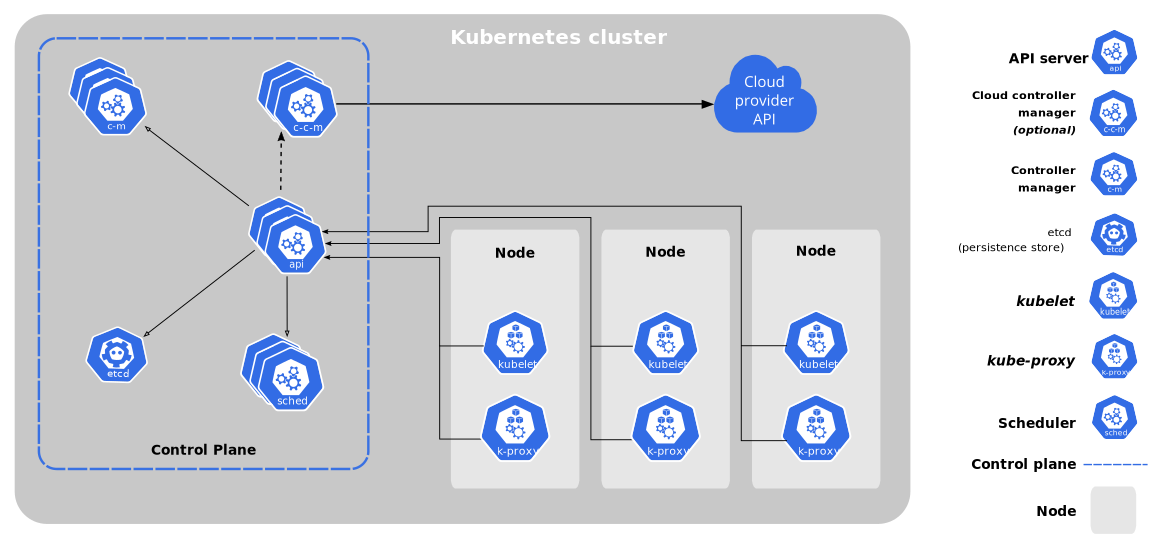
\includegraphics[width=1\linewidth]{figures/2-1-k8s-arch.png}
\caption[Kubernetes cluster architecture diagram]{A diagram\footnotemark of Kubernetes cluster components and processes distributed among them.}

% \medskip
% \begin{minipage}{0.65\textwidth}
% {\footnotesize Depicts Kubernetescluster components and processes distributed among them.\par}
% \end{minipage}

\label{fig:kubernetes:architecture}
\end{figure}
\footnotetext{Source: \url{https://kubernetes.io/docs/concepts/overview/components}, Access: 2021-05-26}
%%%%

With an exposed \emph{Application Programmable Interface (API)} workloads can be dynamically scheduled by any authorized third-party application.
They are represented in a form of a configuration file called \emph{deployment}, which contains details for requested Kubernetes resources such as pods or services.

%%%%%%%



\subsubsection{Pod}\label{s:ProblemDomain:Kubernetes:pod}

A base workload type in Kubernetes is called \emph{pod} and is meant to represent a standalone working process. 
It is used as an abstraction for a set of tightly-coupled containers required to be scheduled on the same worker node.
Although the requests for computing resources for each of the containers within a single pod may differ, they still share the storage with themselves.
In most cases though, a single pod comprises of only one container.

%%%%%%%



\subsubsection{Job}\label{s:ProblemDomain:Kubernetes:job}

Another workload type available is Kubernetes \emph{job}.
This one abstracts the group of pods that should be run together to execute one specific task.
Jobs are often used in situations where there is a need to run a task with a limited execution time and track its completion status and result data.
Also they ensure completion of the task, monitoring statuses of the assigned pods and rescheduling those that have erred until the required number of them have successfully completed.

%%%%%%%



\subsubsection{Kube-scheduler}\label{s:ProblemDomain:Kubernetes:scheduler}

In Kubernetes the responsibility of pod allocation and node assignment belongs to \emph{kube-scheduler}.
The procedure used to determine which node to choose for a specific pod comprises of two actions -- \emph{filtering} and \emph{scoring} \cite{b:Kubernetes-scheduler}.
Filtering process selects candidate nodes that meet pods resource requirements.
When there are no such nodes available at a given moment the scheduled pod must wait for allocation until there is at least one candidate node.
The candidate nodes are then evaluated in the scoring process which determines the best-fitting node for the pod.

It is possible to adjust the scheduler decisions to match the users expectations. 
To limit the possible candidate nodes a pod may have configured additional constraints along its resource requirements.
One of them are node selectors which limit the pool of nodes to those that have defined a specific label on them.
The default Kubernetes scheduler also offers a few scheduling policies to choose from that affect the scoring process.
Additionally, users may also implement their own scheduler components and use them instead of the kube-scheduler \cite{b:Kubernetes-scheduler}.
The only limitation is the new scheduler needs to maintain the filtering and scoring behaviour as a part of the interface.

%%%%%%%


\subsection{Cloud computing}
\label{s:ProblemDomain:Cloud}

The term \emph{cloud computing} is used to describe a group of services with elastic pool of resources available to the end users \emph{on-demand} and settleable based on their usage quota \emph{(pay-as-you-go)} \cite{b:Cloud-Principles-Paradigms}.
In order to distinguish different cloud services they are often classified by their abstraction level as specific service models with the three main being:

\begin{itemize}
  \item{
\emph{Software as a Service (SaaS)} -- the primary resources are provider's applications that run and are managed, transparently to the user
};
  \item{
\emph{Platform as a Service (PaaS)} -- enables deployment of users applications on computing units which abstracts actual physical resources from user, preventing any interaction with underlying infrastructure
};
  \item{
\emph{Infrastructure as a Service (IaaS)} -- a model where users have to configure and manage the infrastructure by themselves, where the base resources are e.g. virtual machines, data storage and network components.
}
\end{itemize}
The abstraction level of a service is related to the number of intermediary layers between the final resource and physical infrastructure.



\subsubsection{Container as a Service}
\label{s:ProblemDomain:CaaS}

Another model of cloud services available in today's clouds is \emph{Container as a Service (CaaS)}.
Relating it to other service models it is classified as one in between of the IaaS and PaaS \cite{b:IBM-CaaS}.
With containers being treated as a primary resource it enables interaction with infrastructure at a higher abstraction level than in IaaS, nonetheless the responsibility for the management process still lies in hands of the end user.
This model offers a more scalable and portable solution to infrastructure management for containerized environments.



\subsubsection{Elastic Kubernetes Service}
\label{s:ProblemDomain:EKS}

An example of an CaaS service is \emph{Elastic Kubernetes Service (EKS)} \cite{b:IBM-CaaS} provided by \emph{Amazon Web Services (AWS)}.
It allows configuration of fully-managed Kubernetes cluster \cite{b:AWS-EKS} in AWS cloud environment.
This means that EKS by itself spans a new cluster, covers the Kubernetes installation process and is responsible for maintaining the Kubernetes control plane outside the cluster's nodes.
The end user is only responsible for initial cluster configuration and requesting workloads on the cluster with Kubernetes API.

\subsection{Workflow}
\label{s:ProblemDomain:Workflow}

Workflow is an application comprising of a set of tasks, where some of them are dependent one on another and all need to be processed in order to complete the workflow's objective and yield the final results.
Each job in such a pipeline may require its own input data to begin execution and returns an output when it ends successfully.
As tasks cannot start without their input, they need to wait for results from other tasks, which creates a dependency relationship.
This allows such applications to be represented in the form of a \emph{Directed Acyclic Graph (DAG)} as shown in \cref{fig:workflow:dag-example}.

Furthermore, not all the jobs in a workflow must perform the same set of operations at runtime.
The pipeline has a layered structure where each layer represents a group of tasks independent of each other.
This allows for a straightforward data-parallel task execution within a single layer. 


%%%%
\begin{figure}[H]
\centering
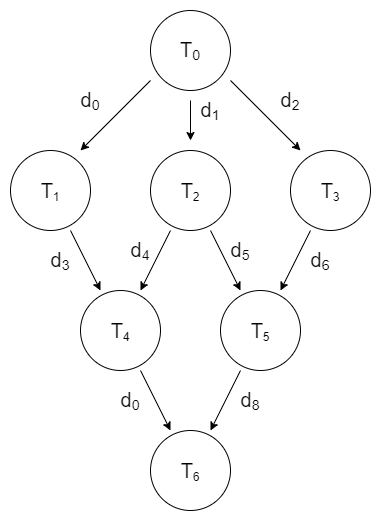
\includegraphics[width=0.3\linewidth]{figures/2-3-dag-example-with-d.png}
\caption[Exemplary workflow application structure]{Exemplary workflow application structure. Tasks are presented as a \emph{T\textsubscript{i}} nodes and dependencies as a \emph{d\textsubscript{j}} edges.}
\label{fig:workflow:dag-example}

% \smallskip
% \begin{minipage}{0.6\textwidth}
% {\footnotesize
% Tasks are presented as a \emph{T\textsubscript{i}} nodes and dependencies as a \emph{d\textsubscript{j}} edges. 
% \par}
% \end{minipage}

\end{figure}
%%%%


There are applications with more than one starting or finishing job, however their representations can have single abstract nodes prepended or appended, in order to match the input for scheduling algorithms.



\subsubsection{Montage}

One of the scientific workflows integrated with Hyperflow system is \emph{Montage}.
It is a toolkit that provides transformations for astronomical images to turn them into custom, science-grade mosaics \cite{b:Montage-url}.
Each transformation is provided as a separate software module \cite{b:Montage} so together they can be piped into a single workflow.



\subsubsection{SoyKB}

The \emph{Soybean Konwledge Base (SoyKB)} is a platform for storing soybean genomics datasets and providing them via an interface for research.
To analyze this data the \emph{PGen workflow} was created allowing analysis on both Linux environment and through SoyKB online submissions \cite{b:SoyKB-workflow-url, b:SoyKB-PGen}.
% The latter environment integration allows execution of the workflow with task containerization.
Being consistent with Hyperflow naming, in this work all mentions of \emph{SoyKB workflow} are in fact referring to the PGen application.




\subsection{Scheduling}
\label{s:ProblemDomain:Scheduling}

The \emph{scheduling problem} is a term referring to a process of arranging tasks and assigning them to selected processing units with goal of workload optimization, e.g. minimize completion time.
To provide a sub-optimal solutions to this NP-complete problem many heuristics have been researched and developed with two main approaches considered -- \emph{static} and \emph{dynamic} scheduling.
The final solutions can be \emph{workflow-aware} which means they take the dag-oriented structure of the workload into consideration during task arrangement.


\subsubsection{Static scheduling}
\label{s:ProblemDomain:StaticSched}

In static scheduling, it is assumed that all requirements are already defined, including task resource demands and information about execution environment with underlying infrastructure.
This approach allows to optimize the workload distribution across all of the computing units.
At the same time it lacks the adaptability to unforeseen changes in resource availability. 


There are multiple categories of static scheduling algorithms, one of them being a \emph{list-based} ones.
The \emph{list-based} algorithms consist of two phases:


\begin{itemize}
  \item{
\emph{prioritization} -- during this phase each task has its the \emph{rank} value calculated and has its priority based off of it. The tasks are then ordered descendingly by their priorities
};
  \item{
\emph{selection} -- in this stage the final sequences of tasks are formed, one for each available computing unit. A sequence binds the tasks to a selected processor and defines their execution execution order that must be followed.
}
\end{itemize}


An example of list-based workflow scheduling algorithm is \emph{Heterogeneous Earliest Finish Time (HEFT)}, where the rank of a task is based on the its computation and communication costs \cite{b:HEFT}.
Another algorithm worth mentioning is a \emph{Predict Earliest Finish Time (PEFT)}.
Despite both algorithms using same parameters in rank calculation process, they have different formulas defined.
The difference comes from PEFT's \emph{Optimistic Cost Table (OCT)} which is used to evaluate the future impact of assigning a given task to specific node \cite{b:PEFT}. \todo{ Może wspomnieć o wynikach porownania PEFT do HEFT z \cite{b:PEFT} ?}



\subsubsection{Dynamic scheduling}
\label{s:ProblemDomain:DynamicSched}

The dynamic approach to scheduling problem concentrates more on an issue of changeability of computing environment, availability of its resources and changes to processors load.
All scheduler's decisions are being made at runtime based on information know only at the exact moment in time.
This makes them more adaptable, but at the same time there is a disadvantage of worse workload optimization than with static scheduling \cite{b:Dynamic-Scheduling-Case-Study}.
Additionally, the dynamic nature makes it a go-to approach for cluster schedulers \cite{b:Tetris, b:Graphene}.



\subsubsection{Task clustering}
\label{s:ProblemDomain:TaskClustering}

Executing a lot of short tasks in a single limited computing environment leads to increase in slowdown and decrease in overall resource utilization.
To address this problem the \emph{task clustering} solutions are used.
The idea behind them is to group the waiting tasks into the multi-element clusters and treat them as a single entity \cite{b:Task-Clustering-Pegasus} during the scheduling process.

There are various approaches to clustering tasks in a workflow.
The ones related to granularity problem are:


\begin{itemize}
  \item{
\emph{horizontal} -- also called a \emph{level-based}, is a clustering solution that forms groups based on the task level of in workflow's DAG representation. In horizontal approach clusters can be composed of entities with the same level
};
\item{
\emph{vertical} -- tasks are grouped only vertically with the child tasks dependent on them or the parent tasks they are dependant on. The problem with vertical clustering is the task resource requirements in the same cluster may differ
};
  \item{
\emph{label-based} -- in this approach all tasks are being labeled by the end user and grouped with other ones that have the same label. Then all the tasks within a single cluster have to be ordered for an execution \cite{b:Task-Clustering-Hybrid-Algorithm, b:Task-Clustering-Pegasus}.
}
\end{itemize}


% Moze przeniesc do osobnej subsection, niekoniecznie zwiazany z schedulingiem ?


\subsection{Hyperflow}
\label{s:ProblemDomain:Hyperflow}

\emph{Workflow Management System (WMS)} is a software responsible for coordinating and supervising workflow execution.
It provides storage layers for data exchange, manages states of the workflow's tasks and handles permissions for waiting jobs to allow them to run only when their dependencies are fulfilled.
One of such systems is \emph{Hyperflow} -- an innovative yet lightweight and simple model for workflow execution \cite{b:Hyperflow}.
Its two main constituents are an engine, which makes all the decisions regarding workload allocation, and an executor that handles assigned workloads within separate processes, monitors their status and reports completion to the engine.


Executors are the supervisors spawned by an engine using a concept Hyperflow functions.
With each one implementing a different workload deployment solution for a specific kind of infrastructure Hyperflow can be used in various computing environments including Kubernetes clusters \cite{b:Hyperflow-k8s-deployment}.
The \cref{fig:hyperflow:architecture} presents an overview of a system architecture in a Kubernetes environment.
Each workflow's task is considered as a separate workload and is represented by a single Kubernetes job.
Its deployement is being requested by the Hyperflow engine through a function that calls the cluster's API.


%%%%
\begin{figure}[H]
\centering
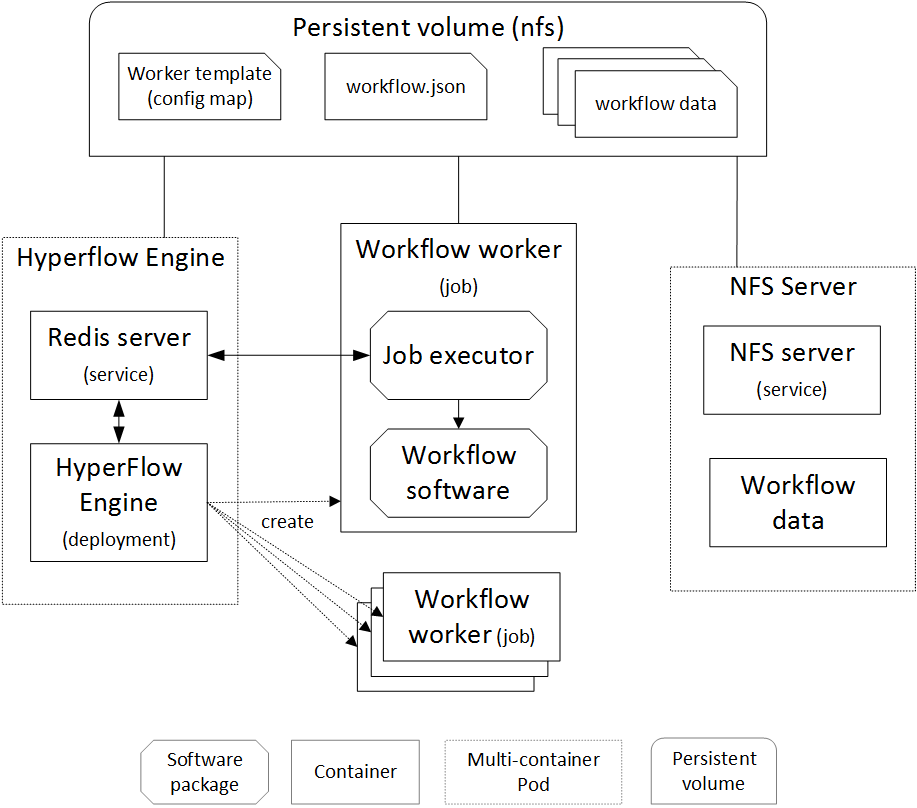
\includegraphics[width=0.6\linewidth]{figures/2-4-hyperflow-k8s-arch.png}
\caption{Hyperflow architecture in Kubernetes cluster}

\smallskip
\begin{minipage}{0.7\textwidth}
{\footnotesize\centering
SOURCE: \cite{b:Hyperflow-k8s-deployment}
\par}
\smallskip
{\footnotesize
One of the cluster's nodes is reserved to be a Hyperflow master node.
Engine's components are deployed on the master node, while tasks are deployed with their executors on the worker nodes.
Workflow data is being exchanged through network file system.
\par}
\end{minipage}

\label{fig:hyperflow:architecture}
\end{figure}
%%%%

The engine allows the tasks performing the same operations to be grouped together and buffered, waiting to be assigned to a single executor instance.
Whenever a task becomes ready to be processed it is being either assigned to a new buffer or is being appended to already existing one, associated with this specific task's operation.
This feature is an implementation of a horizontal task clustering solution and is referred to as \emph{task agglomeration} in Hyperflow nomenclature.

Buffers have configurable maximum sizes and have defined time boundaries for them to wait until they are deployed as a Kubernetes job.
They allow grouping until they are already full or the timeout has been reached.
Such configurations are possible for each workflow's operation.



\thispagestyle{only-cfoot}
\section{Related work}\label{s:RelatedWork}

This chapter presents a few selected works related to the problem of this thesis and provides a review of them.
To address non-uniformity of the problem, works from two separate research areas are included.

% As the research problem thesis' problem 
% To address this non-uniformity this chapter presents related works in both research areas.
% \todo{Refer to related work and criticize shortcomings}


\subsection{Workflow-aware cluster schedulers}\label{s:RelatedWork:Schedulers}

The goal of cluster scheduling is to optimize the allocation of tasks to available computing resources.
There are a few challenges the scheduler may focus on dealing with, such as cost minimization, load-balancing, or fairness.
To successfully schedule DAG-based workloads in cluster environments, schedulers need to be workflow-aware.


One of such schedulers is \emph{Graphene} proposed in \cite{b:Graphene}.
It introduces a two-step approach to scheduling workflows based on the identification of so-called \emph{troublesome tasks} and planning workload execution around them.
First, the tasks are being ordered and then packed and allocated to selected best-fitting cluster resources.
Evaluation of the concept was conducted against other production-grade solutions (e.g. \emph{Apache TEZ}\footnotemark[1]  with \emph{Capacity Scheduler}\footnotemark[2]) on existing DAG-based application workloads \cite{b:Graphene}.
The presented results are remarkable, especially the considerable makespan reduction.
Unfortunately, the outcomes are achieved at the cost of the solution's complexity.
Neither Graphene nor the idea of two-phase scheduling of scientific workflows was adopted and evaluated in Kubernetes environment, to our best knowledge.


Another solution to cluster scheduling is \emph{Tetris} -- a scheduler which uses a greedy approach with multidimensional packing for its decision making process \cite{b:Tetris}.
To support DAG-based workloads, the adjusted version of \emph{Shortest Remaining Time First (SRTF)} algorithm was introduced and integrated with the packing solution.
The proposed concept was evaluated against both \emph{Capacity Scheduler}\footnotemark[2] and \emph{Fair Scheduler}\footnotemark[3] in a simulation with custom created workloads.
Although the declared results lead to an impressive reduction in job makespan, in \cite{b:Graphene} it is claimed that Tetris does not perform well enough when scheduling DAG-structured workflows.
% Lastly, the soulution was not evaluated as a Kubernetes scheduler.

%%
\footnotetext[1]{Apache TEZ: \url{http://tez.apache.org/}, Access: 2021-07-02}

\footnotetext[2]{Apache Hadoop YARN Capacity Scheduler: \url{https://hadoop.apache.org/docs/current/hadoop-yarn/hadoop-yarn-site/CapacityScheduler.html}, Access: 2021-07-02}

\footnotetext[3]{Apache Hadoop YARN Fair Scheduler: \url{https://hadoop.apache.org/docs/r2.9.1/hadoop-yarn/hadoop-yarn-site/FairScheduler.html}, Access: 2021-07-02}
%%

%%%%%%%%
\subsection{Scheduling performance comparison}\label{s:RelatedWork:Performance}

One of the goals of this work is the analysis and juxtaposition of different workflow scheduling approaches.
This includes a comparison of various algorithms in specific computing environments.

The studies of \cite{b:Performance-Analysis-Scheduling-DAG} and  \cite{b:Performance-Comparison-Scheduling-DAG} describe such comparison processes, achieved with simulations run on randomly generated DAG-based workloads.
None of them present information about the underlying infrastructure in detail, the only detail provided is the number of processing units used.
In each work, an analysis was conducted for a different set of state-of-the-art, list-based workflow scheduling algorithms, however, all of them included HEFT and PEFT.
To evaluate the solutions, a few different and important metrics were used, such as schedule length ratio, speedup, and efficiency.
Unfortunately, in both \cite{b:Performance-Analysis-Scheduling-DAG} and \cite{b:Performance-Comparison-Scheduling-DAG} no information was provided about Makespan comparison to evaluate job completion optimization capabilities.
Results from all mentioned works show that PEFT is one of the best available solutions, outperforming other algorithms for most of the covered scheduling criteria.



%%%%%%%%
\subsection{Summary}

None of the reviewed works had conducted an evaluation in Kubernetes cluster which is one of the main goals of this thesis.
Additionally, other than the Graphene scheduler, there is no solution fully addressing the workflow scheduling problem for containerized clusters that achieves good enough results. 
Due to the time constraints of this work, it is impossible to reproduce the same scheduling behaviour as in Graphene and use it as a solution for the experiments.
The algorithm comparison related works lack the data and analysis of the job completion times achieved by the evaluated solutions.



% \include{3-methodology}
\thispagestyle{only-cfoot}
\section{Scheduling DAG-based workloads in Kubernetes}\label{s:SchedHyperflow}
% Scheduling workflows in Kubernetes

% Tutaj, że korzystamy z Hyperflow do workflowów, wymieniamy jakie są opcje i dlaczego pomijamy nadpisywanie kube-schedulera.

% \todo{Outline of solution chapter}
This chapter presents the concept of a solution to scheduling workflow tasks in Kubernetes clusters.
Suggestions to enable task clustering with scheduling are included.

%%%%%%%
\subsection{Analysis of approaches}\label{s:SchedHyperflow:Deliberation}

% Kubernetes scheduler by design does not support static scheduling of workflow tasks for future.
% Its only responsibility is to select the most applicable node for a pod at a given time, depending on the resource requirements.
% To study the impact of preplanning the execution of DAG-based workloads in Kubernetes, the concept for a solution to such a mechanism first needs to be proposed.



% As mentioned in \ref{s:ProblemDomain:Kubernetes:scheduler}, the kube-scheduler does it through the process of filtering and scoring.
% Although the filtering should leave in the node selected in a plan for job execution, the problem becomes more apparent with the scoring procedure.
% It may choose different resources for a pod to run on, depending on the current cluster state. 



%% BEGIN - Deliberation on approaches
There are two obstacles to overcome in scheduling DAG-based workloads on Kubernetes clusters.
The first one regards the proper handling of dependencies between the tasks, ensuring their execution in the right order, imposed by the graph structure.
This is usually one of the liabilities of workflow management systems, and thus can be considered resolved by including their engine in the execution flow.
%
The other obstacle is the prioritization of the tasks available to be run.
In Kubernetes, the default cluster scheduler makes pod allocation decisions in first-come first-served order, based on the time they have been requested to be deployed.
With the current scheduling approach, it is not possible to change the order of pods to allocate, given the sequence of requested workloads and an expected sequence of prioritized tasks are different.
There is an option to assign priority to each requested workload definition, this however would only affect the currently scheduled pods or ones yet waiting for an assignment decision.
Furthermore, this would require a separate entity to be responsible for task ordering, as the priorities would need to be assigned beforehand. 

% Although the filtering should leave in the node selected in a plan for job execution, the problem becomes more apparent with the scoring procedure.
% It may choose different resources for a pod to run on, depending on the current cluster state.

% As mentioned in section \ref{s:ProblemDomain:Kubernetes:scheduler}, the kube-scheduler does it through the process of filtering and scoring.


% Considering all of the mentioned ...

Considering the mentioned issues, to allow workflow-aware scheduling in Kubernetes, it is necessary to first adjust the current solution.
There are two ways to do so, either create another cluster scheduler and use it instead of kube-scheduler or introduce a new separate entity responsible for task scheduling and run both alongside.
The difference between these approaches is in their flexibility.
As mentioned in section \ref{s:ProblemDomain:Kubernetes:scheduler}, the kube-scheduler makes decisions in the process of filtering and scoring, which means the new cluster scheduler would have to be tailored to match this behaviour with both obstacles remaining unsolved.
On the other hand, an approach with a second scheduler requires only the prioritization process to be covered.

In this work, we decided to further explore the second approach as it better fits the needs of our experimental process with the support for interchangeability of scheduling algorithms. The Hyperflow engine was utilized as an workflow execution supervisor, and thus the first obstacle was removed, leaving only the prioritization as a matter of concern.

% \begin{itemize}
%   \item{
% \emph{Create a new cluster scheduler} and use it instead of kube-scheduler. This is the most Kubernetes native approach, however by 
% };
%   \item{
% \emph{Infrastructure as a Service (IaaS)} -- a model where users have to configure and manage the infrastructure by themselves, where the base resources are e.g. virtual machines, data storage and network components.
% }
% \end{itemize}




% !While this may not be a problem for dynamic scheduling strategies, it is a real concern for static algorithms, which plans for CPU assignment and task execution order are expected to be followed.

% Drugim jest realizacja przygotowanego planu przy przypisywaniu podów do zasobów.
% Priorytetyzacja, a nie plan

% Jedną z możliwości jest 


% Kube-scheduler opiera się o filtering i sconring, i jego decyzje mogą się znacznie różnić od tych podjętych przez algorytmu planujące.

% Pomimo mozliwości nadpisania schedulera własnym rozwiązaniem, api pozostałoby niezmienne, a to wymagałoby od takiego schedulera przykładowo wzięcia odpowiedzialności WMS. ...


% Innym rozwiazaniem jest oddzielenie obu tych  od komponentu schedulera k8s ...

% Takie podejście wydaje się być rozsądniejsze, gdyż jest bardziej elastyczne i pozwala badać różne mechanizmy schedulingu bez potrzeby wprowadania kolejnego schedulera.

% Pod

%%%%%%% (stage)
\subsection{Concept of two-phase scheduling}\label{s:SchedHyperflow:PoC}

% \todo{Proof of Concept for DAG Scheduling in K8s}

%%% wrzuc zdjecia wykonan bez i z HEFT / PEFT i opisz przydzial na node'y (lub przykladowy schedule, lub oba)

% inquire
% drop wymiany kube-sched -> instead node-selectory + plugin

% Opisz ze korzystamy z HFlow + wstaw diagram z nodem, engine, plugin i scheduler + przejdz to K8s funkcji + wstaw diagram ze stanami dodanymi przy schedulingu

% Ze na inicjalizacji wyliczany jest plan, a potem w funkcji realizowane sa metody z interfejsu 

% pod z sched jest opcjonalny
%%

% To adopt 
The proposed concept for scheduling DAG-based workloads in Kubernetes consists of two phases, \emph{prioritization} and \emph{assignment}.
It is similar to the abstract idea of two-step scheduling proposed in Graphene \cite{b:Graphene}, which separates these responsibilities of a scheduler into independent steps -- ordering tasks for execution and then assigning resources to each one to run on.
In the prioritization phase, the tasks are being ordered to form an executable sequence.
After that, each of them waits for their turn until they can be executed.
The other phase is responsible for the process of assigning pods to the cluster nodes.
This part is handled entirely by the kube-scheduler.



%%% Przeedytuj zeby było wiadomo, dokładniej co się dzieje

% \begin{itemize}
%   \item{
% \emph{prioritization} -- in this phase, the tasks are being prioritized to form an executable sequence. After that, they are held in waiting before they can be executed 
% };
%   \item{
% \emph{assignment} -- a phase responsible for the process of assigning pods to the cluster nodes. It is handled by kube-scheduler.
% }
% \end{itemize}
% It is similar in an abstract idea to the two-step scheduling proposed in Graphene \cite{b:Graphene}, which separates these responsibilities of a scheduler into independent steps -- ordering tasks for execution and then assigning resources to each one to run on.


A conceptual representation of the necessary scheduling components for Hyperflow system in Kubernetes is shown in \cref{fig:solution:k8s-plugin-arch}.
The scheduler responsible for prioritization is included as a plugin to the Hyperflow engine.
The full implementation of the scheduler\footnotemark[1] and a template\footnotemark[2] to configure a new one are both shared for future reference.

\footnotetext[1]{Scheduler implementation: \url{https://github.com/Kmiet/hyperflow-dag-scheduler-plugin}, Access: 2021-07-20}
\footnotetext[2]{Scheduler template: \url{https://github.com/hyperflow-wms/hyperflow-simple-scheduler}, Access: 2021-07-20}

%%% Diagram node, z engine + pligun + sched
% Podpis diagraamu mowi ze sched jest opcjonalny i moze byc odpalony w podzie

%%%%
\begin{figure}[H]
\centering
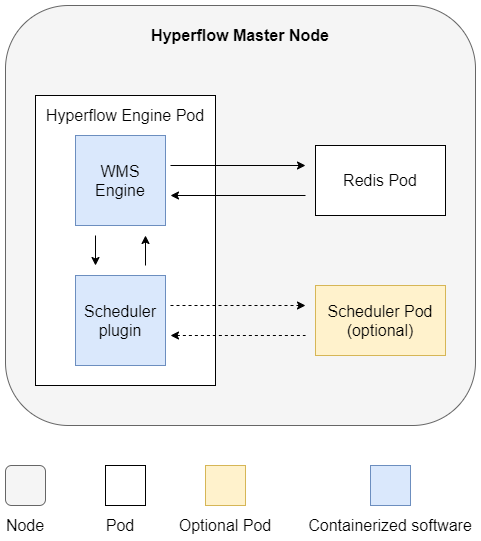
\includegraphics[width=0.5\linewidth]{figures/4-1-HflowPluginArch.png}
\caption[Concept of scheduling in Hyperflow]{Hyperflow master node in Kubernetes with scheduling components. The scheduler pod is an optional container deployed as a Kubernetes service. It is used to facilitate inclusion of scheduling algorithm with engine incompatible implementations.}

% \medskip
% \begin{minipage}{0.67\textwidth}
% {\footnotesize The scheduler pod is an optional container deployed as a Kubernetes service. It is used to facilitate inclusion of scheduling algorithm with engine incompatible implementations. \par}
% \end{minipage}

\label{fig:solution:k8s-plugin-arch}
\end{figure}
%%%%
\clearpage


% The plugin .. \todo{wrzuc zdanie o pluginie?}.
To be able to communicate scheduling decisions from the plugin to the kube-scheduler, all necessary information has to be sent in the workload deployment configuration.
% both scheduler decisions with each other \todo{(funkcje kubernetesa + pliki deployment -> node selector)}.
In \cref{fig:solution:k8s-states-single} all states of a modified single Hyperflow Kubernetes function are presented.
For static scheduling, a kube-scheduler is only responsible for pod-to-node assignment based on the provided node selectors.
Decisions on the availability of computing resources and their allocation are being handled by one of the scheduling algorithms.
Each resource identifier can be translated by the scheduler plugin to the matching cluster node selector.

\footnotetext[3]{HEFT Implementation: \url{https://github.com/mackncheesiest/heft}, Access: 2021-07-20}
\footnotetext[4]{PEFT Implementation: \url{https://github.com/mackncheesiest/peft}, Access: 2021-07-20}

%%% Tu diagram ze schematem działania schedulera -> interfejs WMS i sched -> K8s funkcja
% opis

%%%%
\begin{figure}[H]
\centering
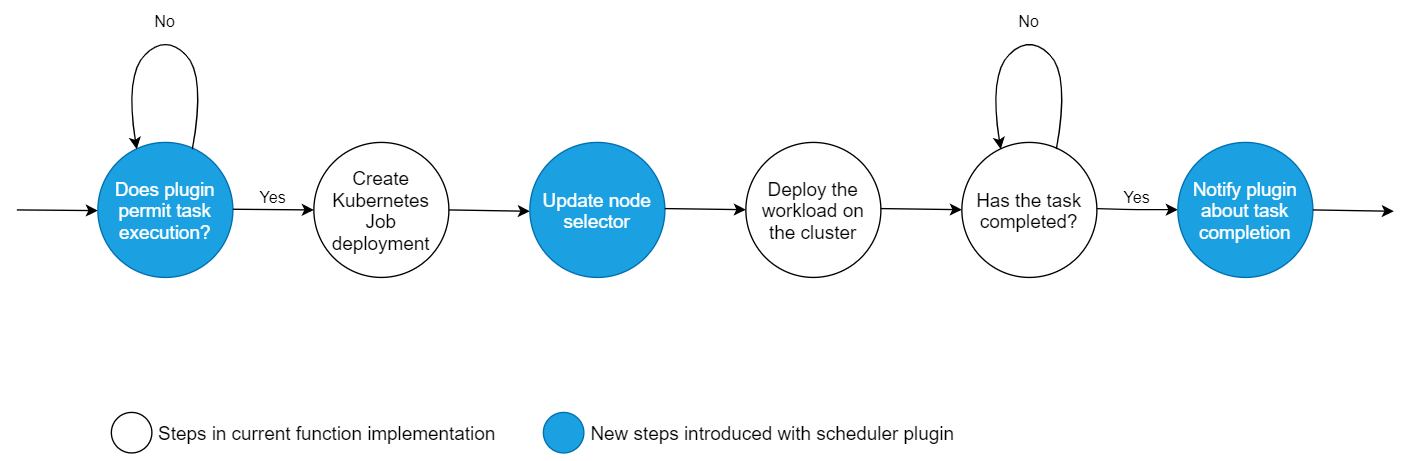
\includegraphics[width=1\linewidth]{figures/4-1-K8sFunction-2.png}
\caption[Adjusted Hyperflow function for Kubernetes workload scheduling]{States of an adjusted Hyperflow function for Kubernetes workload scheduling. The permissions from the scheduler plugin are a mechanism to ensure the correct order of execution for a single specific computing unit.}

% \medskip
% \begin{minipage}{0.65\textwidth}
% {\footnotesize The permissions from the scheduler plugin are a mechanism to ensure the correct order of execution for a single specific computing unit.\par}
% \end{minipage}

\label{fig:solution:k8s-states-single}
\end{figure}
%%%%


% The proposed concept for scheduling DAG-based workloads in Kubernetes is based on an idea similar to the two-step scheduling presented in Graphene \cite{b:Graphene}, which separates these responsibilities of a scheduler into independent steps -- ordering tasks for execution and then assigning resources to each one to run on.

% It is similar to the two-step scheduling proposed in Graphene \cite{b:Graphene}, which separates these responsibilities of a scheduler into independent steps -- ordering tasks for execution and then assigning resources to each one to run on.

For the experiment purposes, a pod with a static scheduler has been deployed and run as a Kubernetes service.
It supports a HEFT\footnotemark[3] and PEFT\footnotemark[4] algorithms for scheduling workflows.
To be able to plan the whole execution process, it is assumed that the necessary data of computation and communication costs for tasks are already provided at the workflow start.
With that input, a schedule is being computed using one of the selected algorithms.
The plugin then respects the order of task execution from the returned plan and grants permission for execution only for one task at a time on a single computing unit.

% -> Tu cos, pewnie wstep do omowienia planu lub nic


%%% Tu obrazek z planem wykonania prostego workflowu

% -> Tu cos lub nic


%%% Tu obrazek z wykonaniem prostego workflowu


The differences between a preplanned schedule and execution trace come from the lack of control over assignment to a specific computing unit (\cref{fig:solution:sched:plan-vs-trace}).
Therefore, on each subsequent execution, a container may have assigned a locally different processor, but of the same kind in terms of a physical resource.
For example, a pod may run on different cores of the same CPU.
This is guaranteed by the processor-to-node-selector translation, done within the scheduler plugin, which ensures a pod to be assigned and run on the same cluster.

%%%%
\begin{figure}[H]
\begin{subfigure}{1\textwidth}
\centering
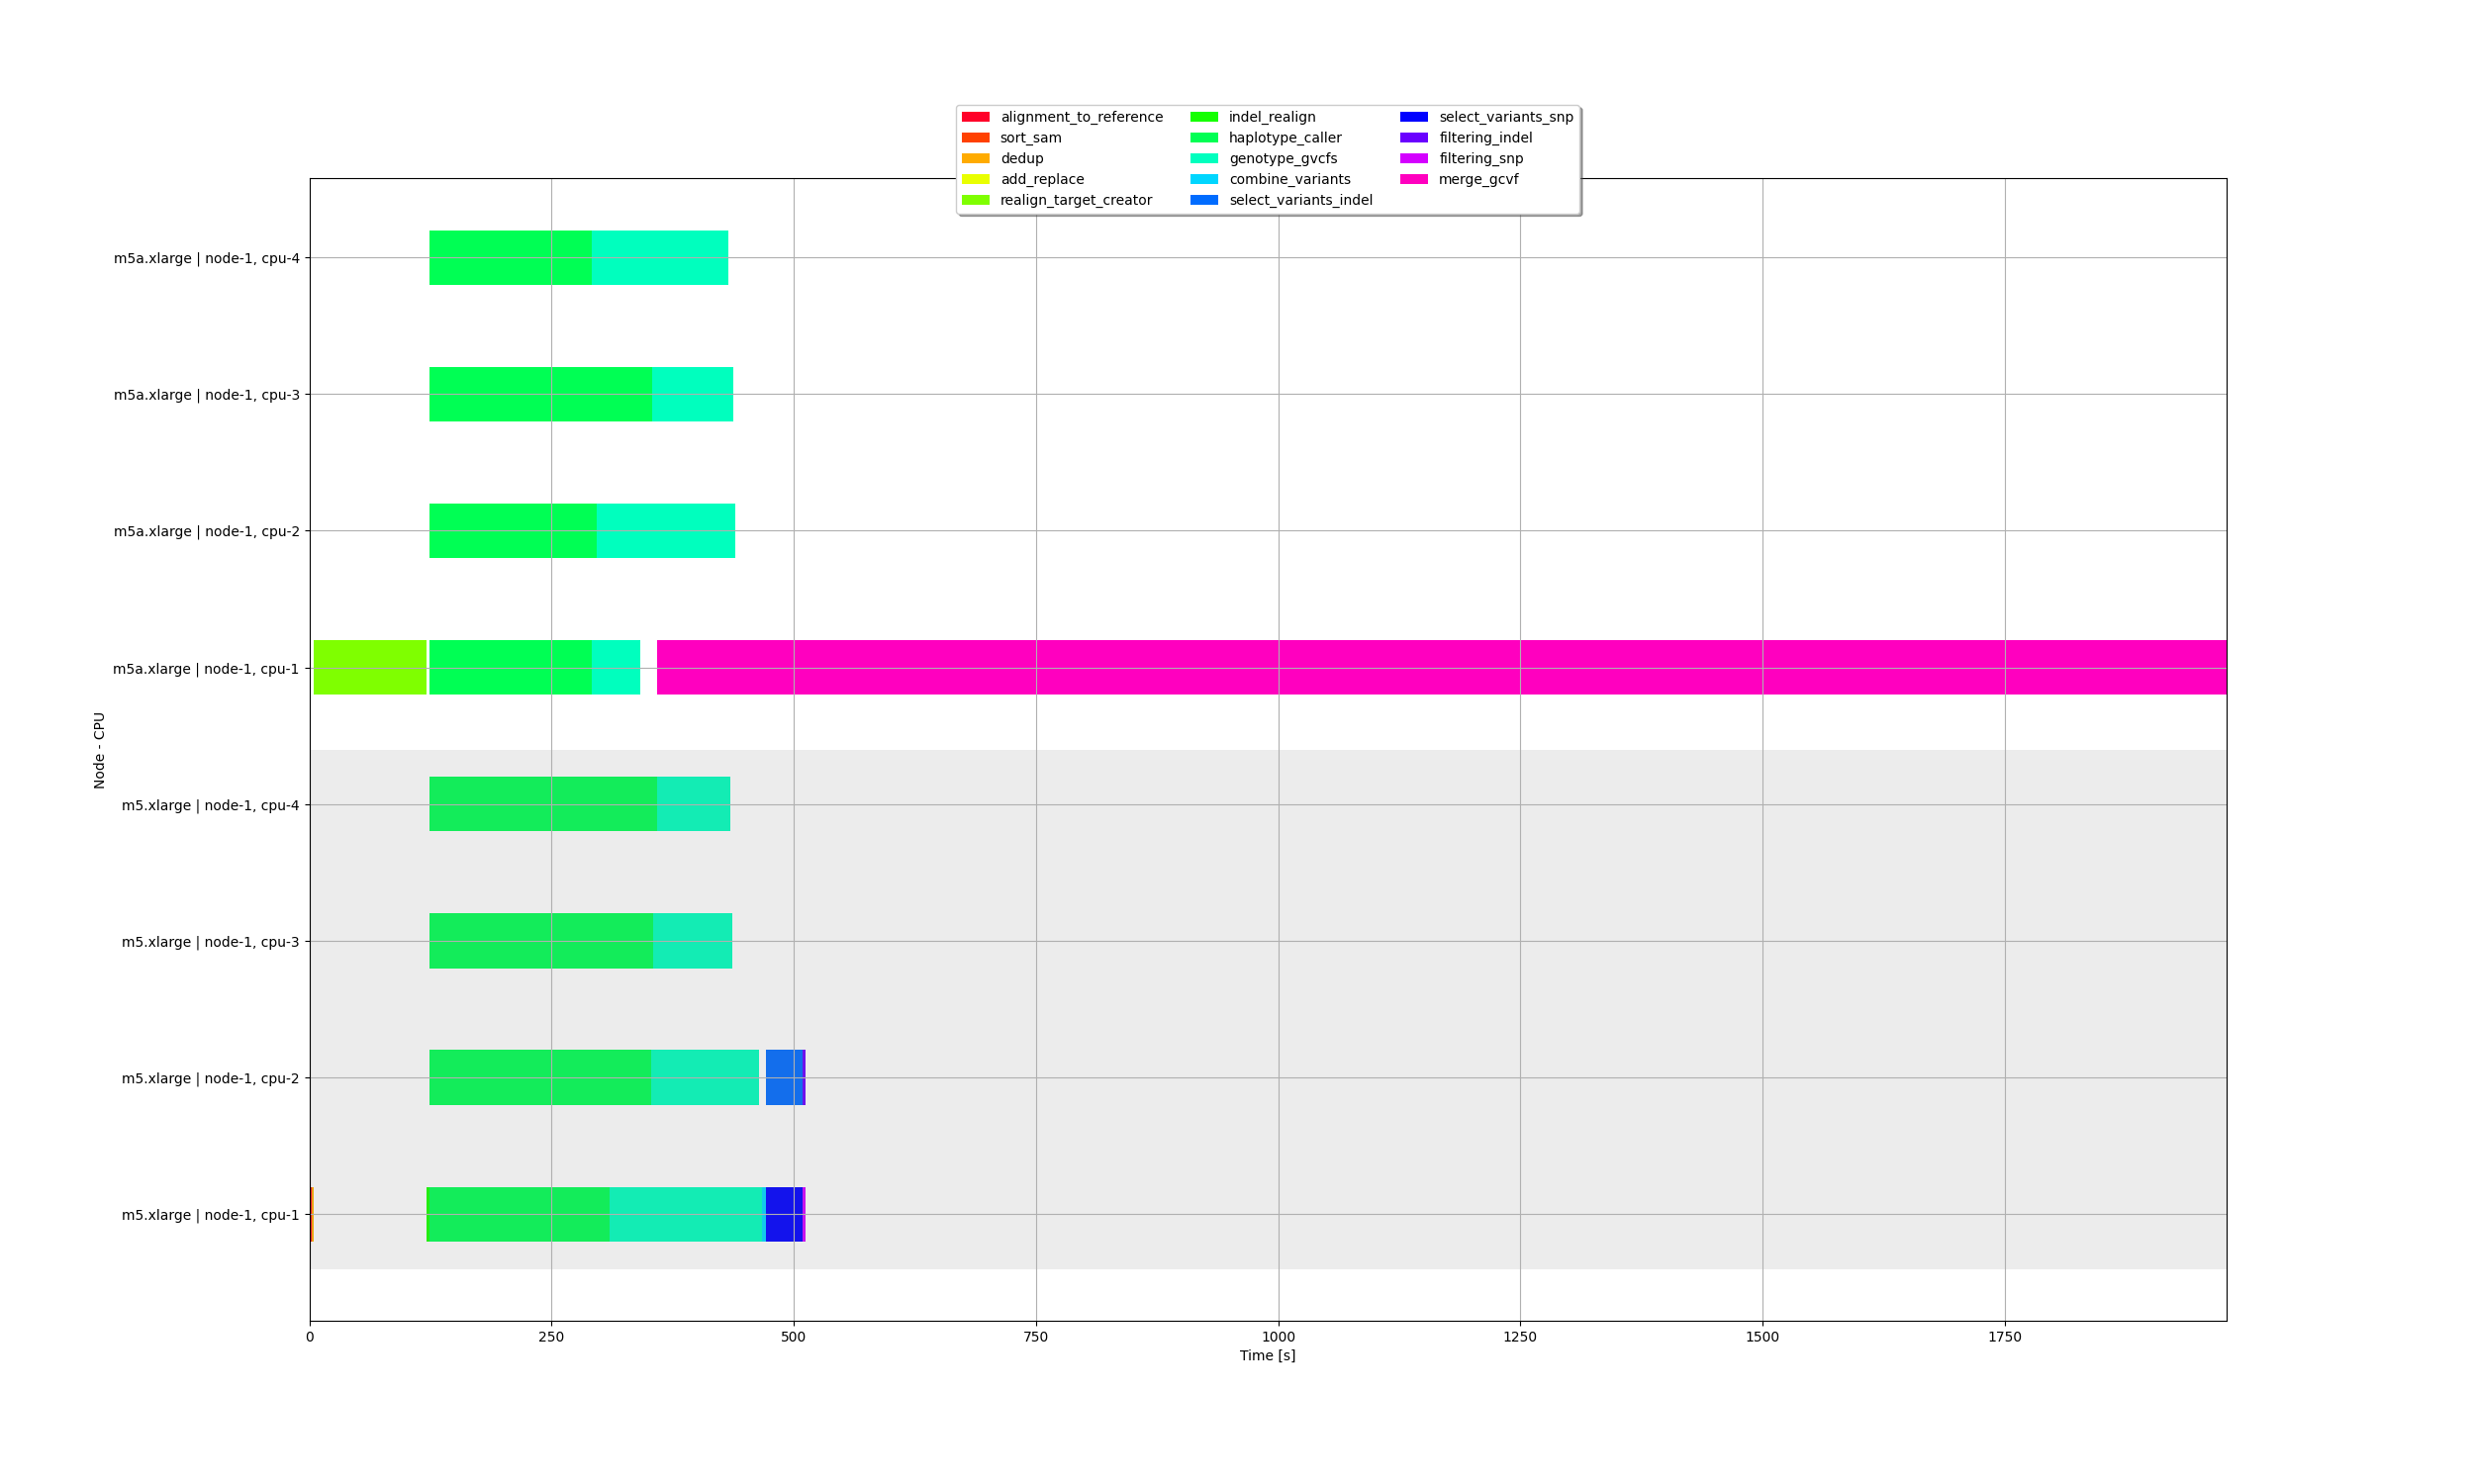
\includegraphics[width=1\linewidth]{figures/5-2-soykb_heft.png}
\caption[ScheduleOnly]{An examplary schedule computed with HEFT algorithm.} 
% \todo{Zmienić diagram na plan wykonania}}
\label{fig:solution:sched:plan}
\end{subfigure}
\begin{subfigure}{1\textwidth}
\centering
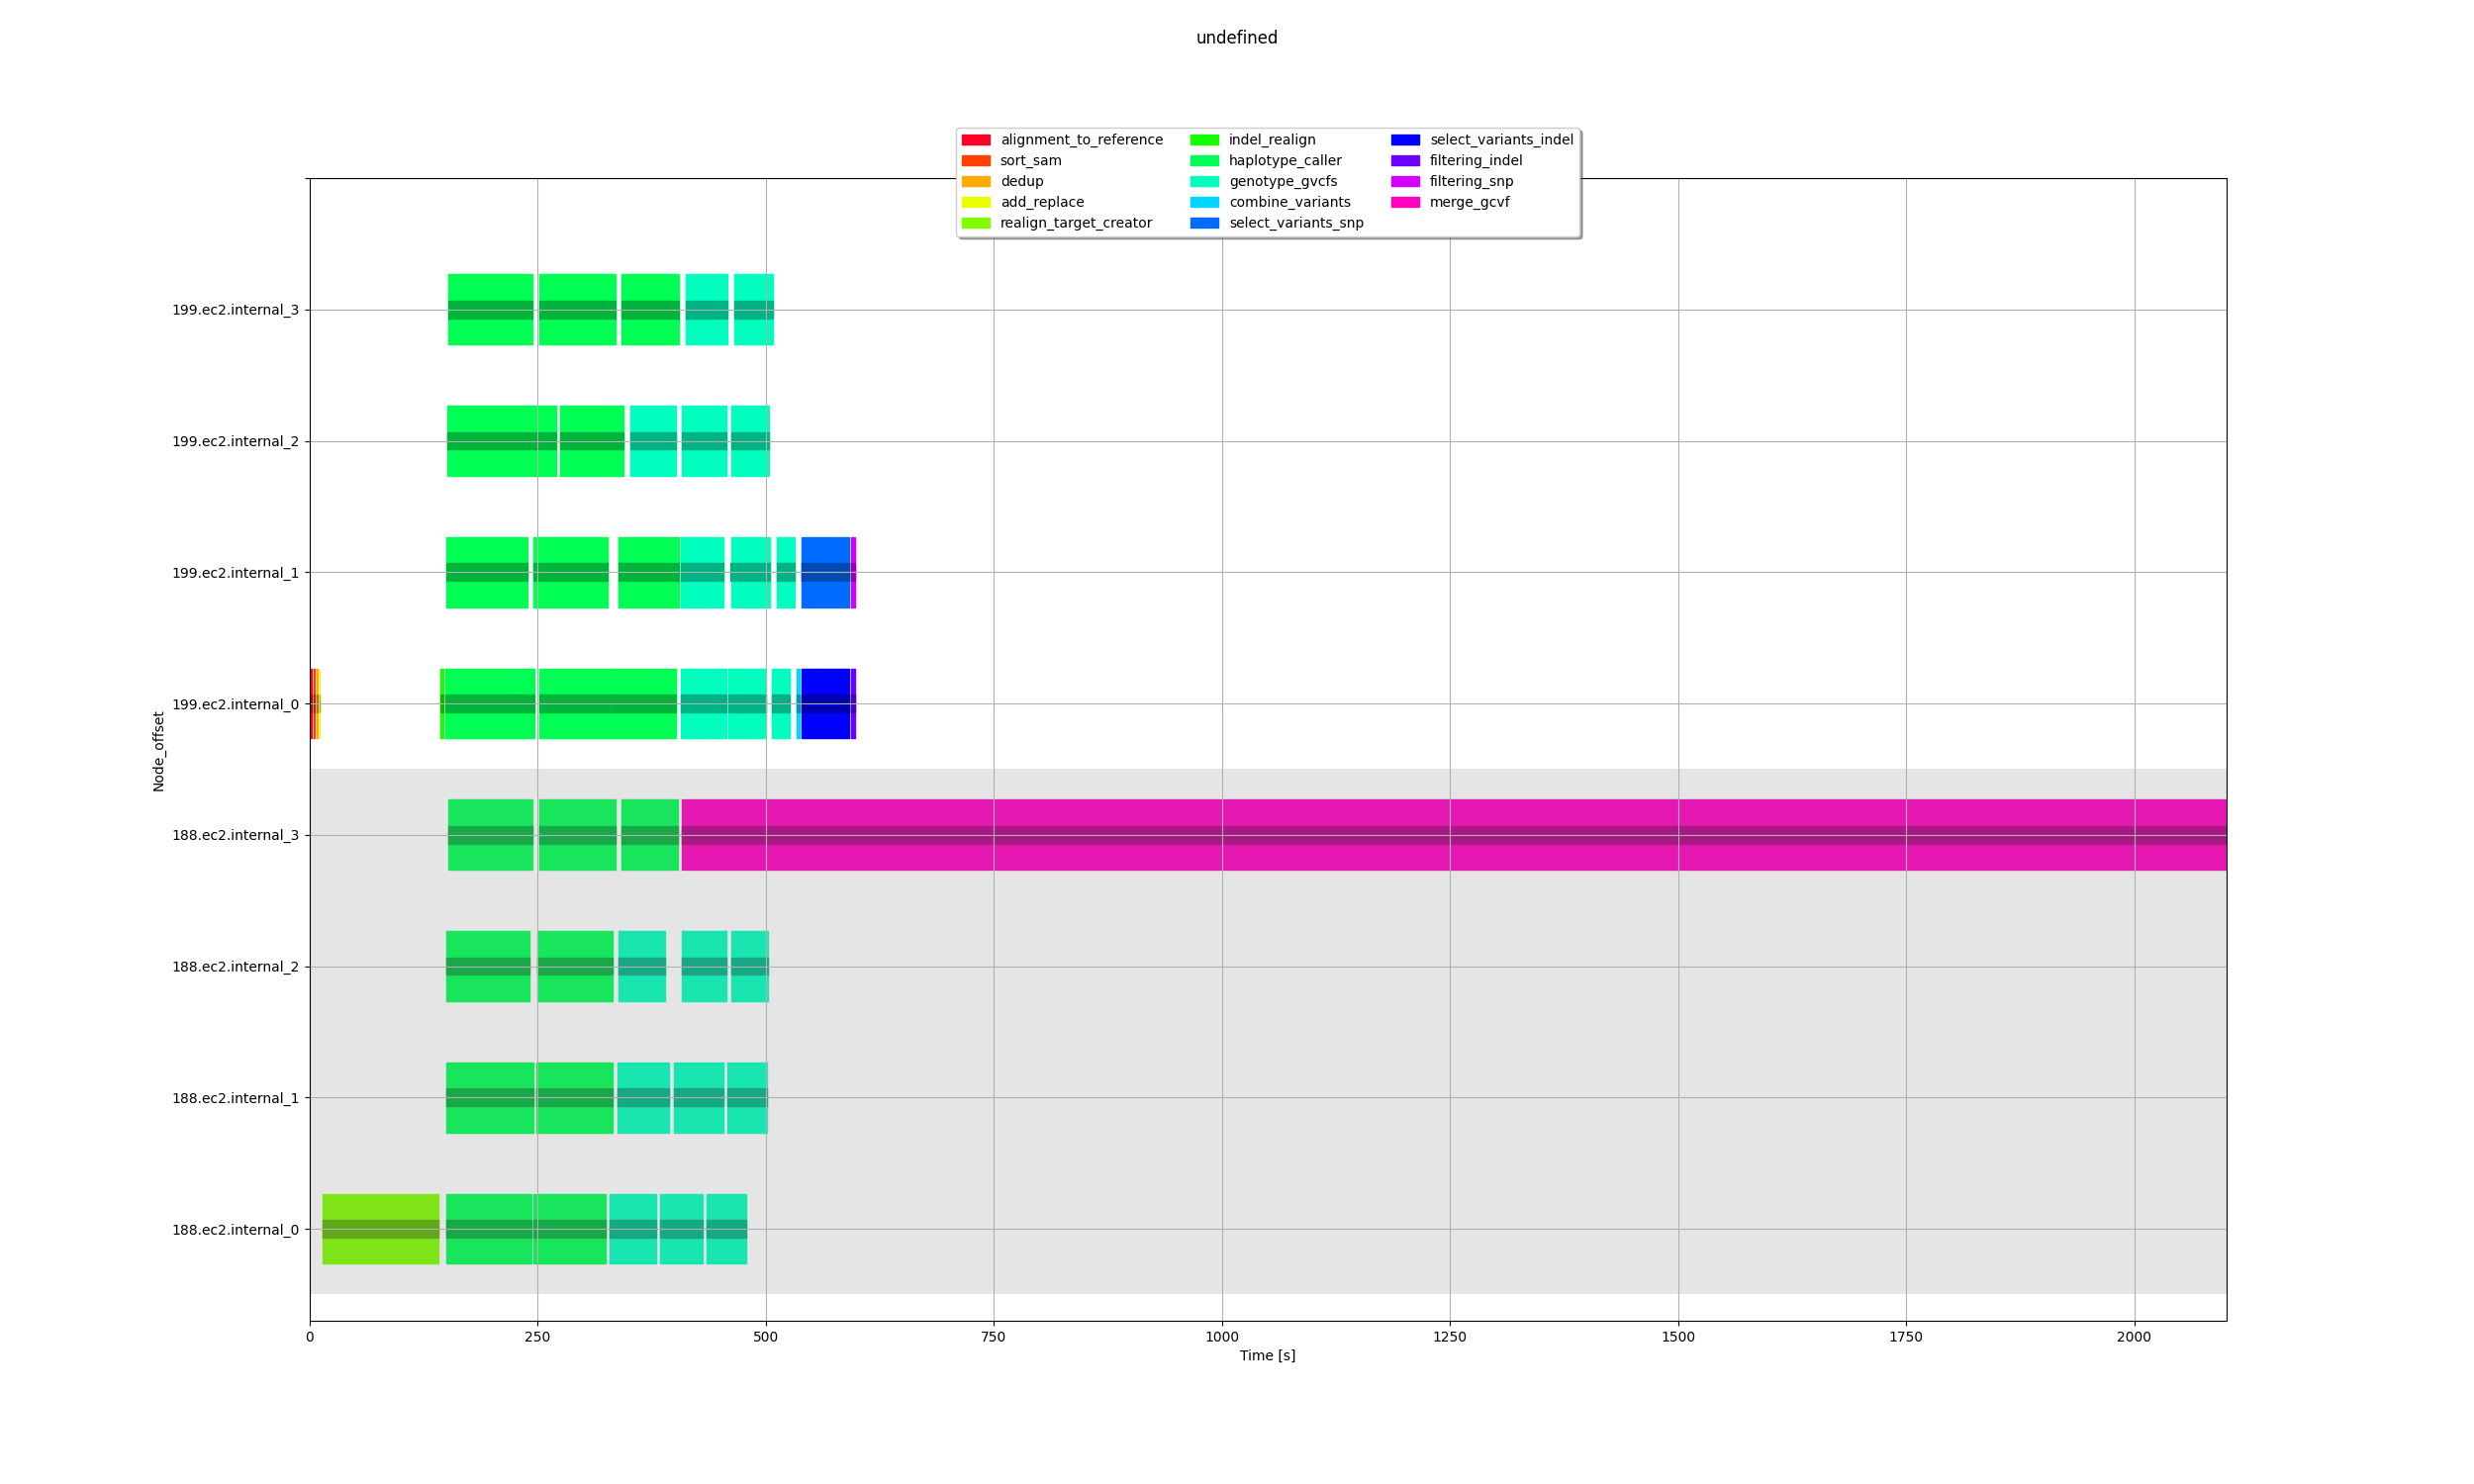
\includegraphics[width=1\linewidth]{figures/4-1-NoAgglo-HEFT.png}
\caption[ScheuleHEFT]{Execution trace for the computed plan from \cref{fig:solution:sched:plan}.}
\label{fig:solution:sched:heft}
\end{subfigure}
\centering

\caption[Differences between computed schedule and execution trace]{Differences in task to processor assignment between schedule and execution trace.}

% \medskip
% \begin{minipage}{0.75\textwidth}
% {\footnotesize Having no limitations on maximum buffer sizes allows creation of a single container with longer lifespan instead of multiple ones for a short periods of time. \par}
% \end{minipage}

\label{fig:solution:sched:plan-vs-trace}
\end{figure}
%%%%


\subsection{Adaptation of task clustering}\label{s:SchedHyperflow:Agglomeration}

%% można opisać phase-opt jako vertical clustering, ale odrzucić


%% this chapter zamiast work?
An expansion of the scheduling problem described in this work is task clustering.
In Hyperflow, \emph{job agglomeration} is managed through the use of \emph{functions} as it is mentioned in section \ref{s:ProblemDomain:Hyperflow}.
However, the current approach with a single task buffer has a few limitations that are not compatible with the presented scheduling solution.
% The states  are shown in \todo{\\cref{}}.

% w Hyperflow Jest ścisle zwiazany z implementacja w wms.
% Dokonano modyfikacji w celu przebadania wersji ze schedulingiem.


% Obecna wersja (diagram?) -> Pliki konfiguracyjne. -> jeden bufor -> ustalony rozmiar bufora -> horyzontalnie


% Adaptowana (diagram stanów) -> automagiczne -> bufor per cpu -> maksymalna objętość -> minimalizacja ilości tworzonych kontenerów -> horyzontalnie -> istnieje możliwość wertykalnej (phase opt), ale kontenery mogą być rózne, więc lepiej nie 


% Since the experiment is being run with Hyperflow engine in Kubernetes cluster, it has been decided not to change the solution entirely.
To adopt the idea of clustering into the scheduling concept, the number of active buffers used in the process has been adjusted to the number of available computing units.
This allows to agglomerate jobs within a preplanned task sequence associated with a given processor.
The diagram in \cref{fig:solution:k8s-states-buffer} presents the states of an modified Hyperflow buffering function for Kubernetes jobs. 

%%% diagram stanów

%%%%
\begin{figure}[H]
\centering
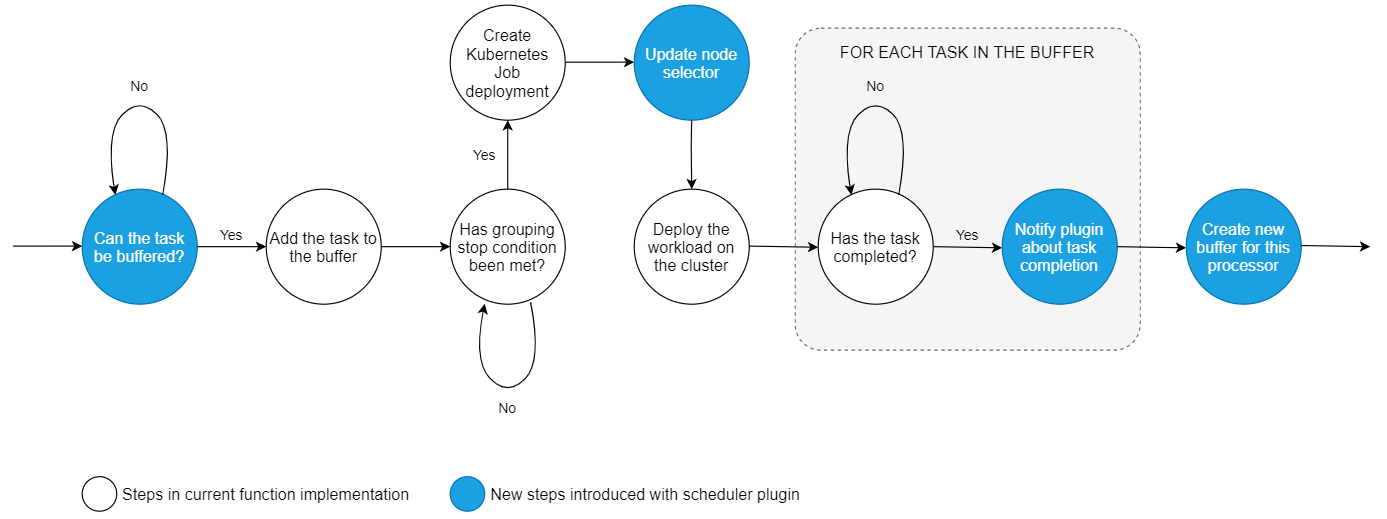
\includegraphics[width=1\linewidth]{figures/4-2-K8sBufferFunction.png}
\caption[Adjusted Hyperflow function for scheduling clusterized workloads]{States of an adjusted function for scheduling clustered tasks as Kubernetes jobs.}

% \medskip
% \begin{minipage}{0.67\textwidth}
% {\footnotesize The diagram presents states in a processor specific context a task specific buffering flow.
% diagram contains states eac permissions from the scheduler plugin are a mechanism to ensure the correct order of execution for a single specific computing unit. \par}
% \end{minipage}

\label{fig:solution:k8s-states-buffer}
\end{figure}
%%%%

% With these adjustments, a conceptual behaviour has not changed.

The task clusterization approach is still horizontal, although it happens only in the context of a single computing unit.
This means the tasks still are being buffered only with the other ones that run the operation.
In the current solution, the buffers require a configuration for their maximum task capacity.
It is set to prevent the possible imbalanced resource consumption that could happen when a majority of tasks from the same horizontal level are grouped into a single buffer.
Utilization of all available resources, or at least the possibility of their inclusion during the execution process, are guaranteed by the schedule.
Therefore, there is no longer a need to setup limits on the maximum buffer size.
This could help to reduce the overhead for workload containerization during the workflow execution, which will be inquired during the analysis of experimental results.
To better comprehend the differences between the two, the example traces from \cref{fig:solution:agglo:traces} present a workflow execution with both approaches.




%%%%
\begin{figure}[H]
\begin{subfigure}{1\textwidth}
\centering
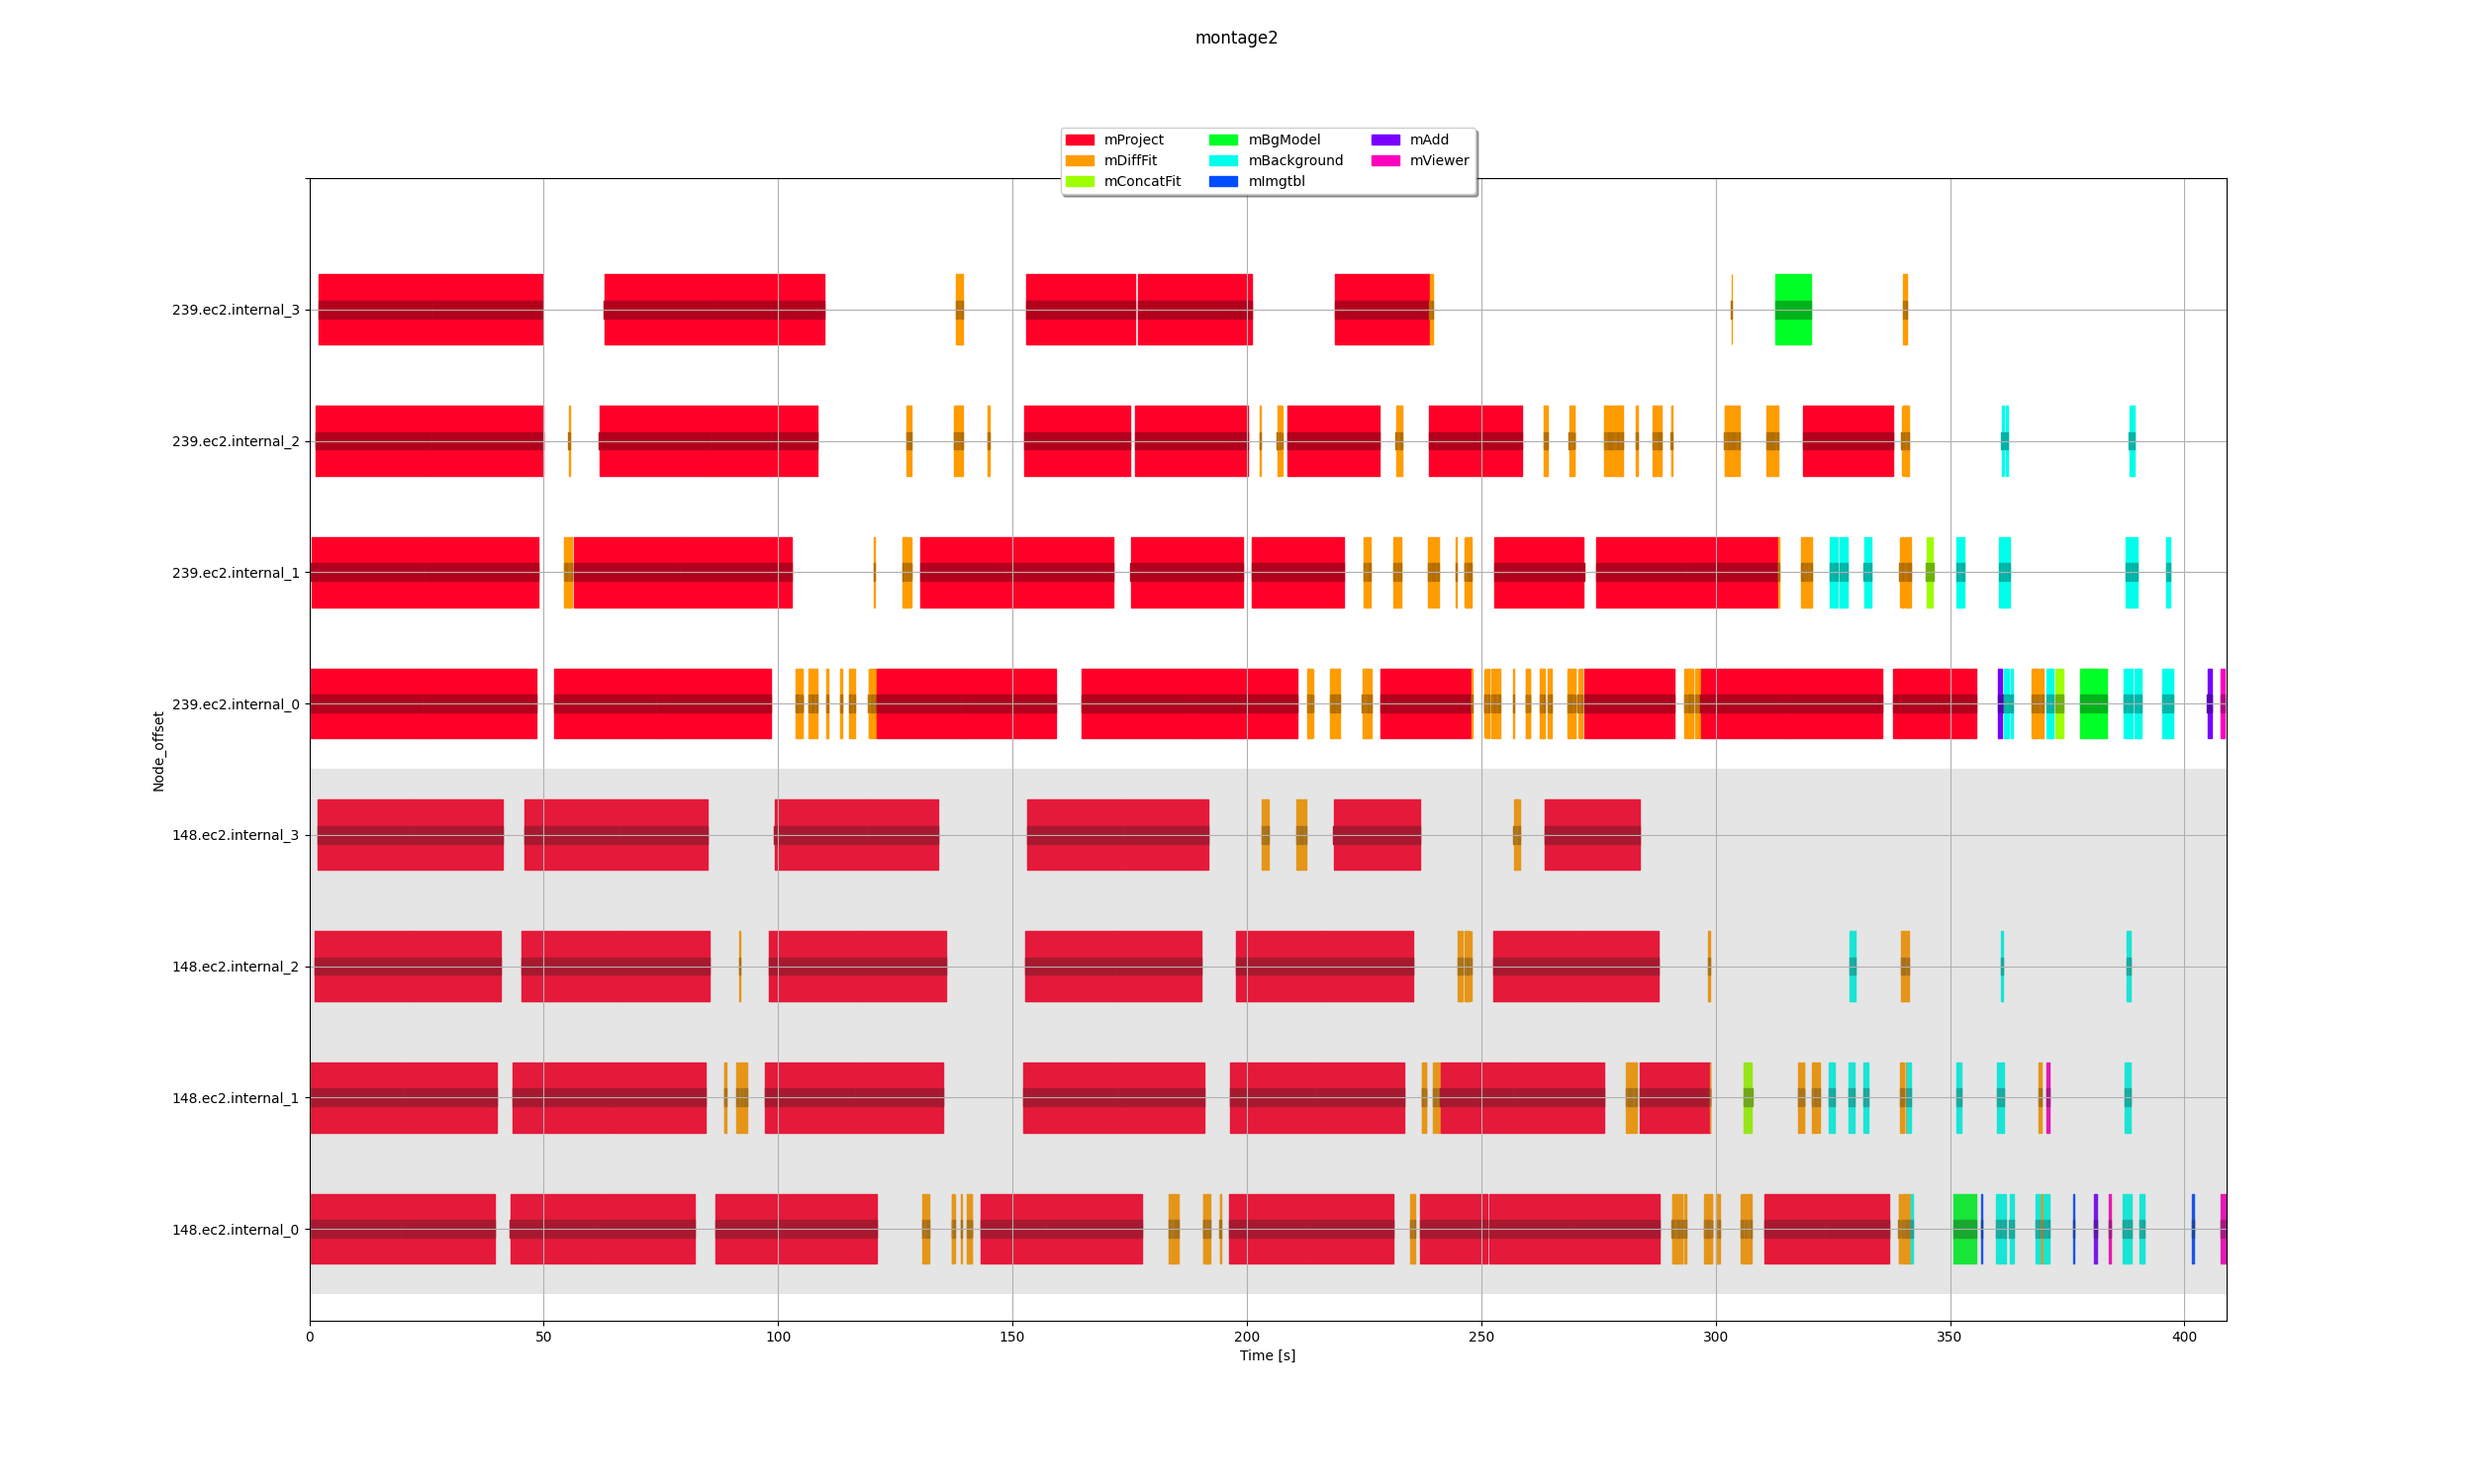
\includegraphics[width=1\linewidth]{figures/4-2-AggloEMPTY.png}
\caption[Agglo EMPTY]{Standard job agglomeration in Hyperflow.}
\label{fig:solution:agglo:empty}
\end{subfigure}
\begin{subfigure}{1\textwidth}
\centering
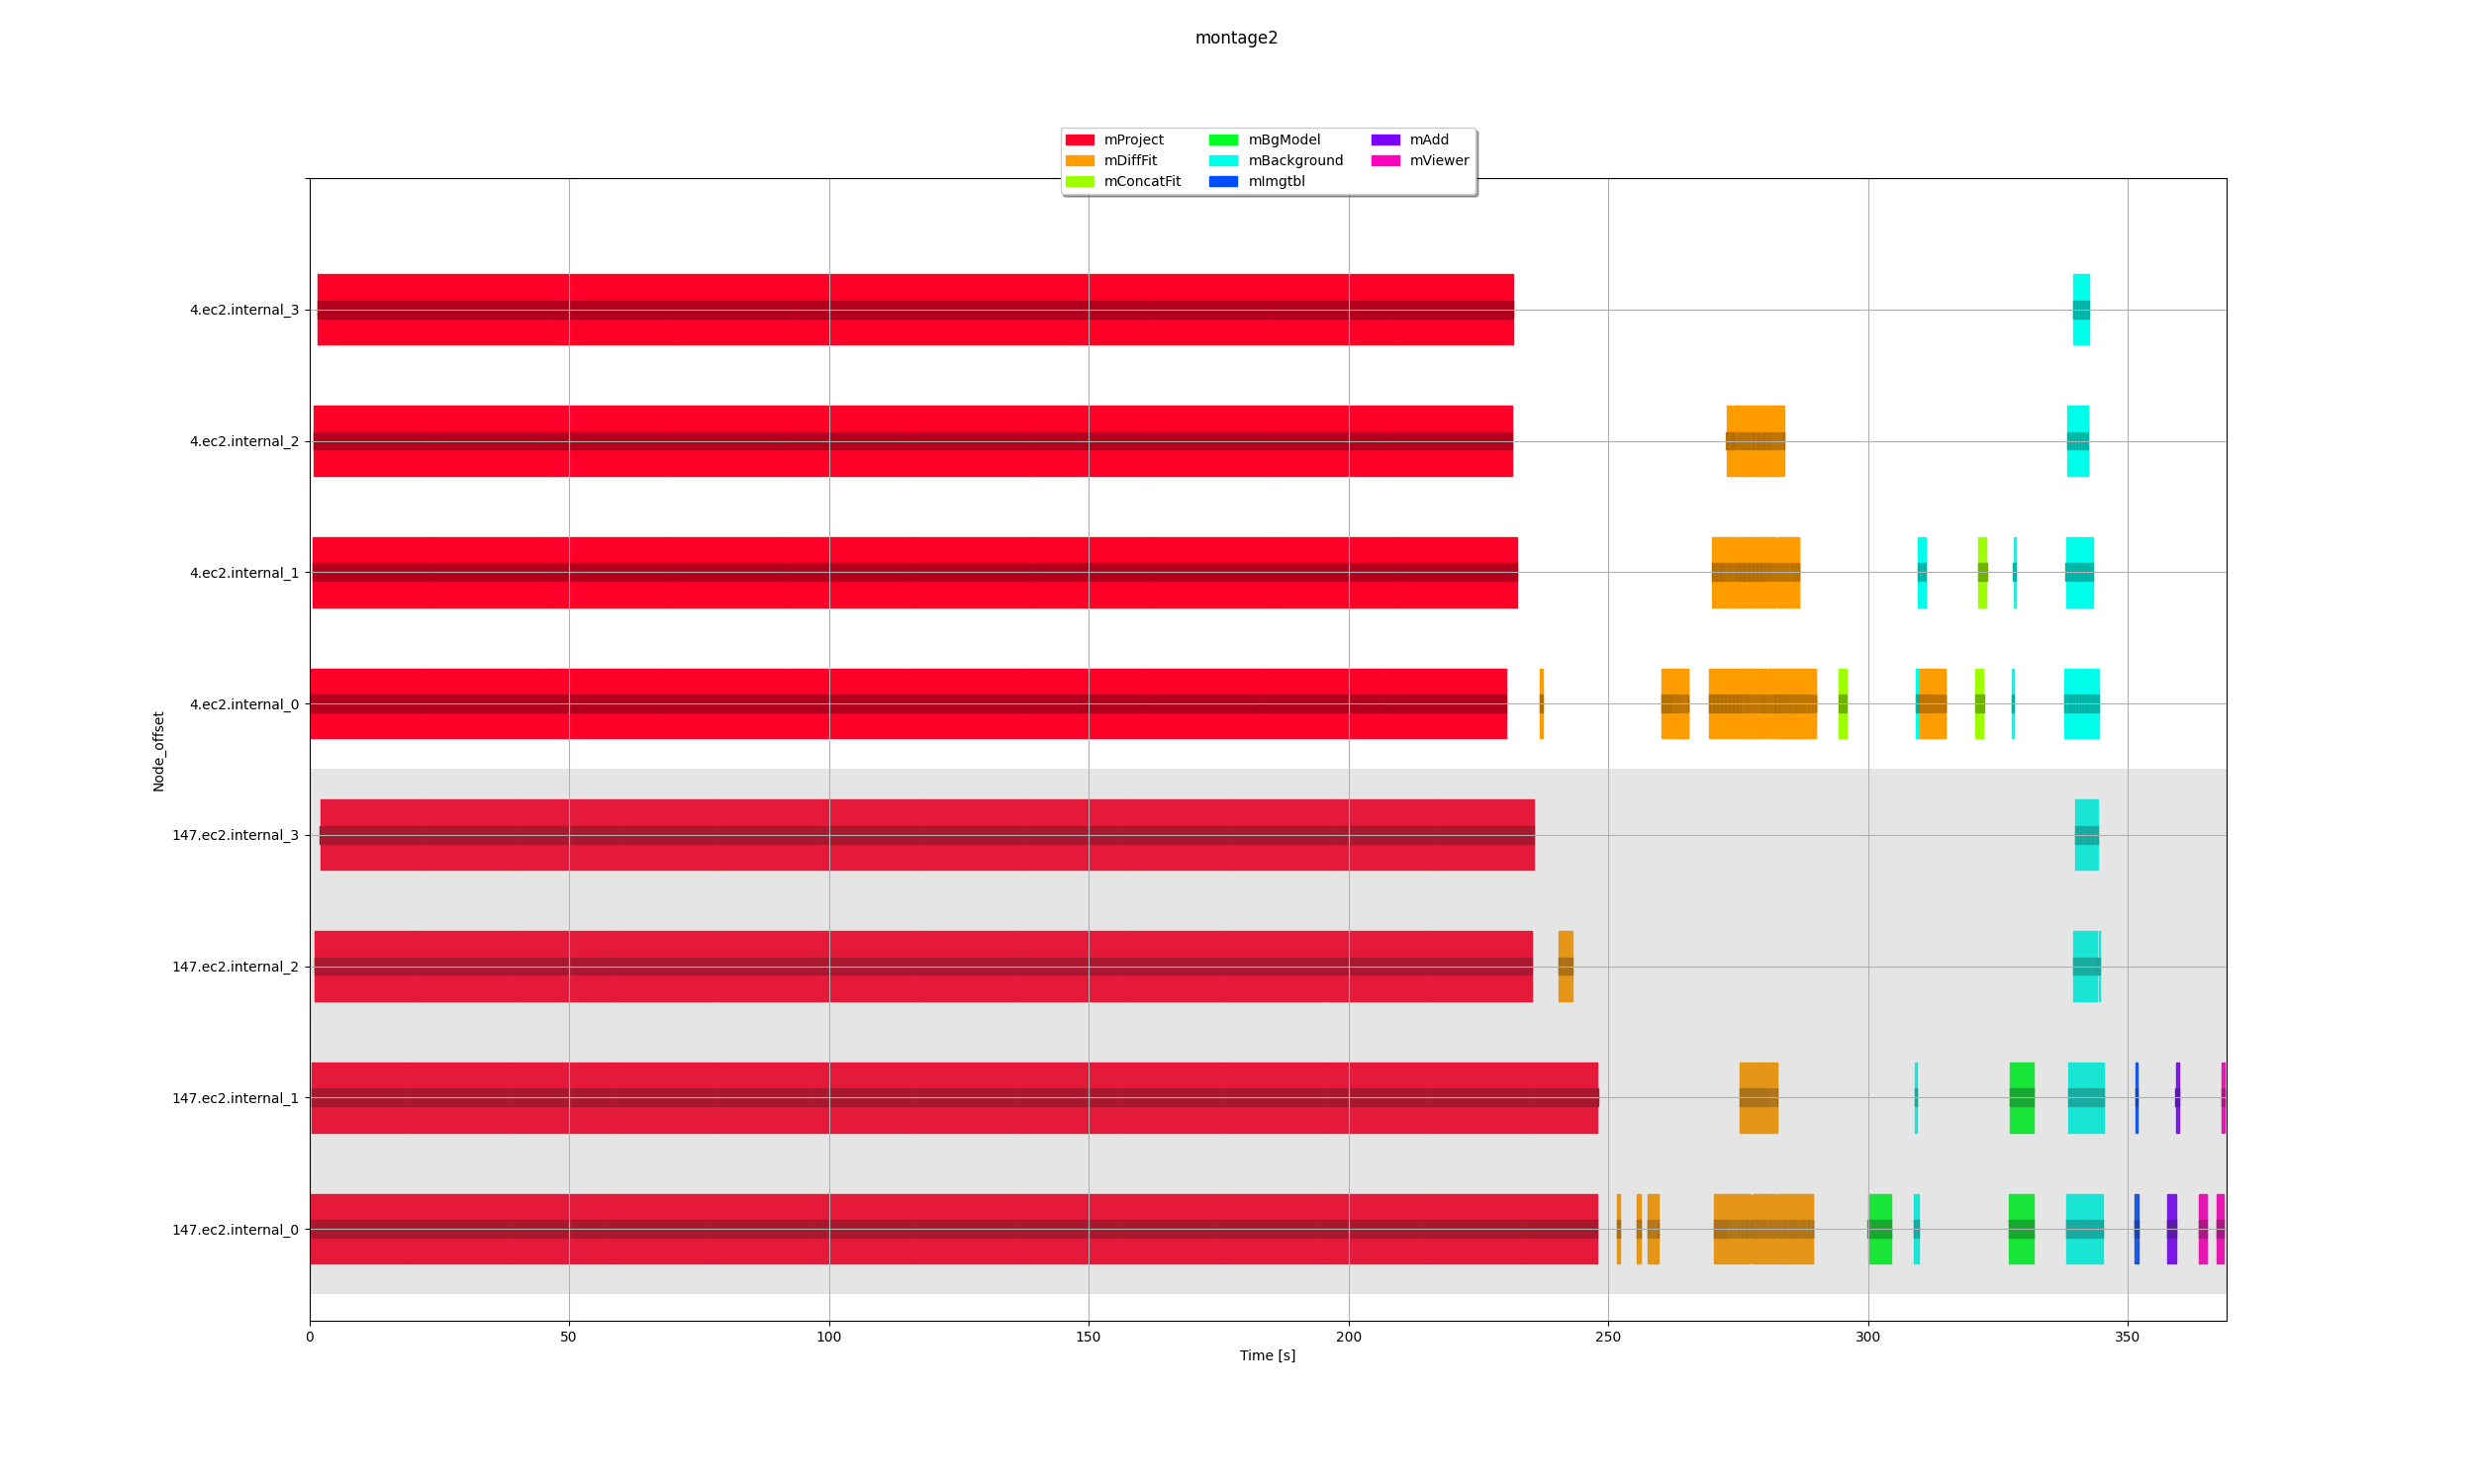
\includegraphics[width=1\linewidth]{figures/4-2-AggloHEFT.png}
\caption[Agglo HEFT]{Modified agglomeration after scheduling with HEFT.}
\label{fig:solution:agglo:heft}
\end{subfigure}
\centering

\caption[Differences in execution traces with task clustering]{Comparison of execution traces with different task clustering approaches. Having no limitations on maximum buffer sizes allows creation of a single container with longer lifespan instead of multiple ones for a short periods of time.}

% \medskip
% \begin{minipage}{0.75\textwidth}
% {\footnotesize Having no limitations on maximum buffer sizes allows creation of a single container with longer lifespan instead of multiple ones for a short periods of time. \par}
% \end{minipage}

\label{fig:solution:agglo:traces}
\end{figure}
%%%%
\thispagestyle{only-cfoot}
\section{Experiment setup}\label{s:ExperimentSetup}

\todo{Write a section outline}
% Comparative experiment

% Agglomeration config, algorithm inputs ?

\subsection{Environment}\label{s:ExperimentSetup:Environment}



\subsection{Metrics}\label{s:ExperimentSetup:Metrics}
\thispagestyle{only-cfoot}
\section{Evaluation}\label{s:Evaluation}

\todo{Outline of experiment evaluation}

% robimy 3 zestawienia (Kube-sched, HEFT, PEFT) dla 3 workflow (SoyKB, Montage 0.25, Montage) w każdym subsection

%%%%%%%
\subsection{Scheduling in Hyperflow}\label{s:Evaluation:HyperflowScheduler}

\todo{Evaluation with task clustering turned off}



%%%%%%%
\subsection{Scheduling with Task clustering }\label{s:Evaluation:Agglomeration}

\todo{Experiments with task agglomeration}



\subsubsection{Job agglomeration by operation}

\todo{Agglomeration - current solution}



\subsubsection{Job agglomeration by operation - no buffer limit}

\todo{Agglomeration - current solution}



\subsubsection{Phase optimization}

\todo{Agglomeration with phase optimization}



\subsection{Summary}

\todo{All experiments summary}
\thispagestyle{only-cfoot}
\section{Conclusions and future work}\label{s:Conclusions}

\todo{Sum up the realized goals and describe future objectives}

%%%


%%% FIGURE LIST
\clearpage % TODO: check if necessary
% \thispagestyle{only-cfoot}
% \cleardoublepage % to ensure that the page reference is correct
% \thispagestyle{empty}
\phantomsection
\addcontentsline{toc}{section}{\listfigurename}
\listoffigures
\thispagestyle{only-cfoot}
\clearpage % TODO: check if necessary
% \thispagestyle{empty}

%%%


%%% ALGORITHMS
% \begingroup
% 	\let \clearpage \relax % to suppress page break

% 	\cleardoublepage
% 	\addcontentsline{toc}{chapter}{\listalgorithmname}
% 	\listofalgorithms
% \endgroup

%%%


%%% BIBLIOGRAPHY
\nocite{*} % forces bibtex to include all citations, whether or not they were referred to in the paper

\thispagestyle{only-cfoot}
% \cleardoublepage
\phantomsection
\addcontentsline{toc}{section}{Bibliography}
\renewcommand{\refname}{Bibliography}
\bibliographystyle{bib-style}
\bibliography{bibliography}


% Clear double page with no styling at the end
\clearpage
\thispagestyle{empty}
\cleardoublepage

%%%

\end{document}
